%%%%%%%%%%%%%%%%%%%%%%%%%%%%%%%%%%%%%%%%%%%%%%%%%%%%%%%%%%%%%%%%%%%%%%%%%%%%%%%%
% EmoManifold — RAL / IEEE conference manuscript draft (English version)
% Translated from emotion_manifold.tex; source-of-truth for facts/numbers remains
% the Chinese draft. Compile from RAL/:  xelatex emotion_manifold_en.tex
% (or pdflatex, since no CJK packages are required in this version)
%%%%%%%%%%%%%%%%%%%%%%%%%%%%%%%%%%%%%%%%%%%%%%%%%%%%%%%%%%%%%%%%%%%%%%%%%%%%%%%%

\documentclass[letterpaper, 10 pt, conference]{ieeeconf/ieeeconf}

\IEEEoverridecommandlockouts
\overrideIEEEmargins

\usepackage{amsmath,amssymb}
\usepackage{graphicx}
\usepackage{booktabs}
\usepackage{cite}
\usepackage{url}
\usepackage{dblfloatfix}

\title{\LARGE \bf
Emo-H2A: Driving Robot Faces Directly from LLM Hidden States at Token Rate
}

\author{Author Name$^{1}$ and Author Name$^{2}$%
\thanks{$^{1}$Affiliation TBD. {\tt\small email@domain.edu}}%
\thanks{$^{2}$Affiliation TBD. {\tt\small email@domain.edu}}%
}

\begin{document}

\maketitle
\thispagestyle{empty}
\pagestyle{empty}

%%%%%%%%%%%%%%%%%%%%%%%%%%%%%%%%%%%%%%%%%%%%%%%%%%%%%%%%%%%%%%%%%%%%%%%%%%%%%%%%
\begin{abstract}
The face is the most natural channel for conveying emotion in human--robot interaction. Current robot faces are driven by a discrete emotion label, not by the LLM's internal affective state during generation. We propose Emo-H2A (hidden-to-actuation), which maps hidden states to facial actuator commands during decoding and removes that intermediate label. We instantiate it as EmoManifold, a training-free projection and mapping pipeline. On a 29-DoF robot face, token-level actuation follows within-utterance affect relative to turn-level discrete labels, and the face updates during generation rather than only after the reply is complete.
\end{abstract}

%%%%%%%%%%%%%%%%%%%%%%%%%%%%%%%%%%%%%%%%%%%%%%%%%%%%%%%%%%%%%%%%%%%%%%%%%%%%%%%%
\begin{figure*}[t]
    \centering
    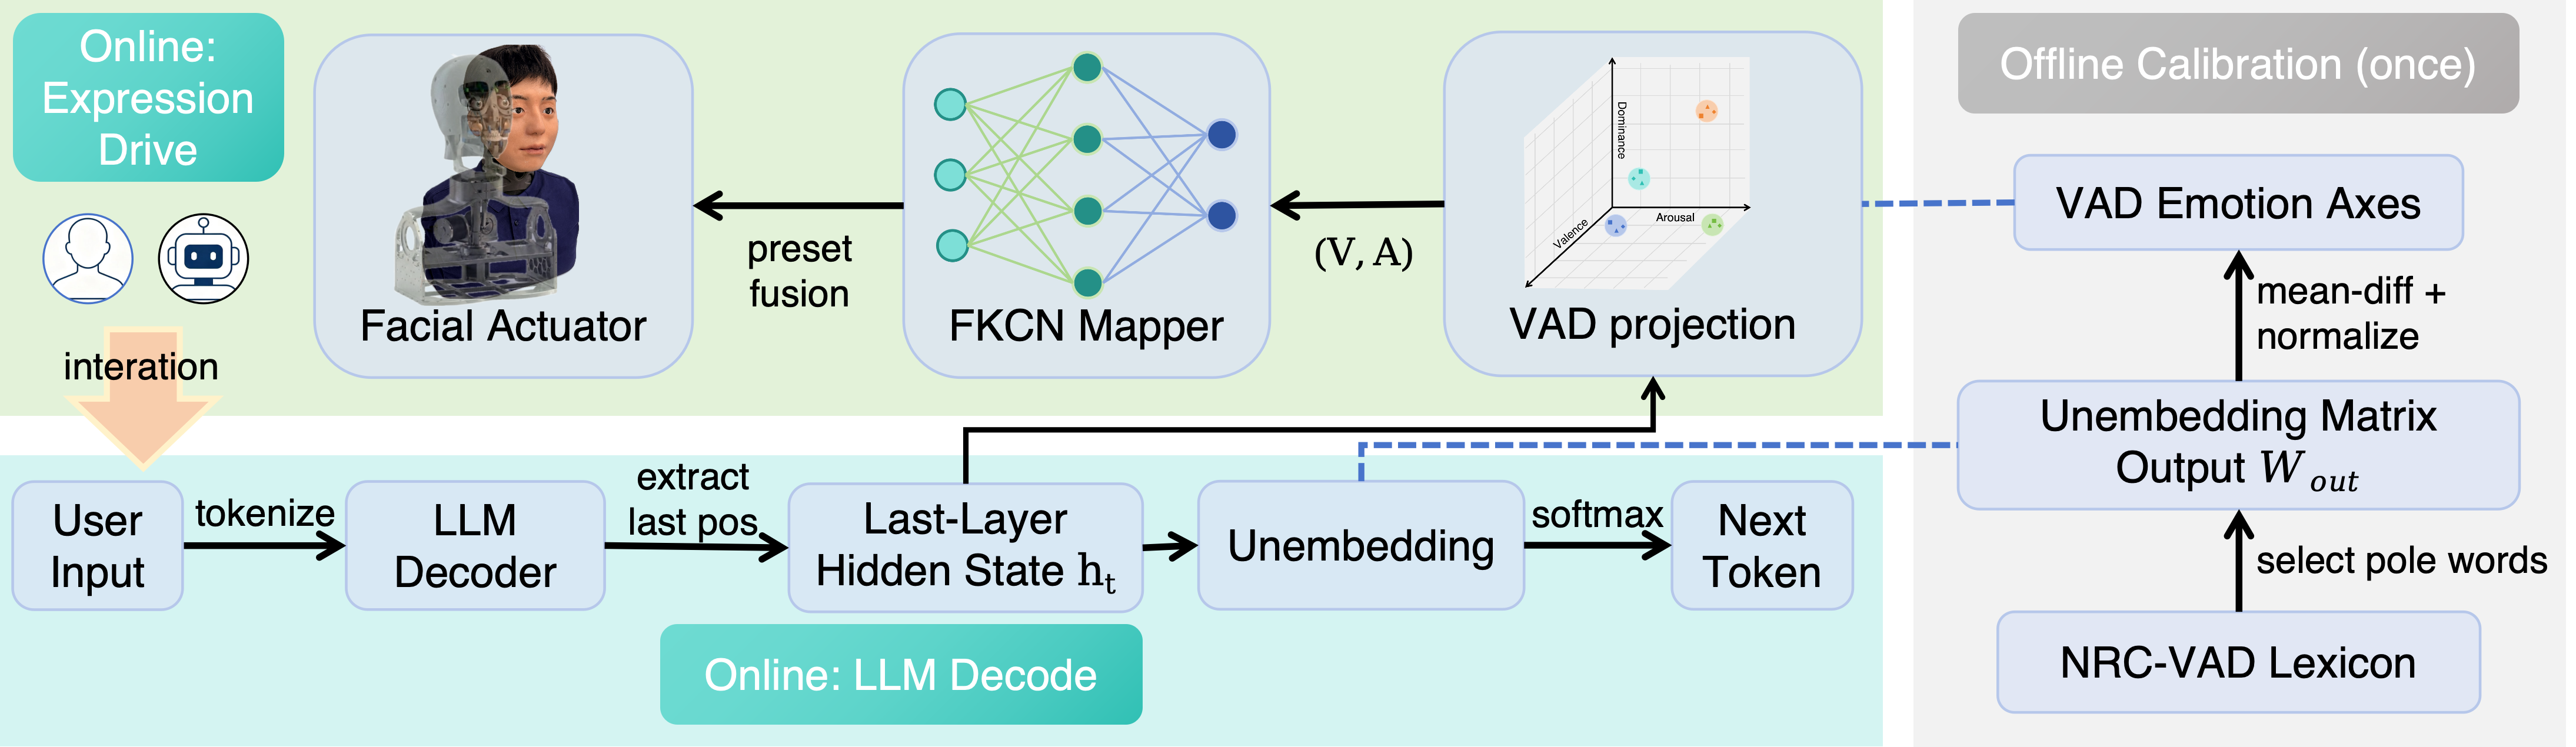
\includegraphics[width=\textwidth,keepaspectratio]{fig/fig1.png}
    \caption{Overview of EmoManifold. Online decoding (bottom): user input is tokenized and passed through the LLM decoder; the final-layer, last-position hidden state $\mathbf{h}_t$ is extracted and unembedded to obtain the next token. Online expression driving (top): $\mathbf{h}_t$ is projected onto valence--arousal--dominance (VAD); its valence--arousal (VA) components are mapped by a Fuzzy Kohonen Clustering Network (FKCN) into seven-dimensional expression weights, fused with presets to drive the facial actuators. Offline calibration (right): NRC-VAD pole words and the unembedding matrix $\mathbf{W}_{\mathrm{out}}$ construct the affective axes once, offline and training-free.}
    \label{fig:1}
\end{figure*}

\section{INTRODUCTION}

``It's written all over your face.'' As people speak, subcortical pathways continuously express underlying emotional states as facial microexpressions, so that affect stays tightly coupled to speech~\cite{ledoux1996emotional}. A machine that converses as naturally as another person---one whose face moves with what it is saying---has long been an aspiration for robotics. Large language models and high degree-of-freedom (DoF) facial hardware now make companionship robots deployable~\cite{ahmed2024companionship}, and give us a chance to take a real step toward that aspiration.

Current robot faces are driven by a discrete emotion label, not by the LLM's internal affective state during generation. LLM-driven systems such as FurChat, Mishra et al., and Xpress produce an emotion label for the reply and map it to a preset expression~\cite{cherakara2023furchat,mishra2023realtime,antony2025xpress}. Work on hidden states shows that affect is linearly readable, but that readout has stayed in offline analysis or in interventions on text generation, and has not been connected to a body~\cite{tigges2024sentiment,reichman2026emotions}. Neither line puts the model's internal affect directly on the face.

This gap narrows in three steps. Continuous expression spaces have long been used in facial robots, as in Kismet's Affect Space~\cite{breazeal2002designing}, but those spaces were not driven by language generation. LLM-driven faces connect expression to a generated reply, yet still assign one discrete label to the whole turn~\cite{mishra2023realtime,antony2025xpress}, so the face cannot follow a change inside the sentence. Turn-level methods, however fine the label, wait until the reply is complete before the first update, so the face cannot move while the model is still speaking.

To address these problems, we propose Emo-H2A (hidden-to-actuation), which maps LLM hidden states to facial actuator commands during decoding and removes the intermediate emotion label. To our knowledge, it is the first paradigm to close this loop on a physical face. We instantiate it as EmoManifold, a training-free projection and mapping pipeline. On a 29-DoF robot face, token-level actuation follows within-utterance affect relative to turn-level discrete labels, and the face updates during generation rather than only after the reply is complete. To foster further research, we will open-source the code. In summary, our main contributions are:
\begin{itemize}
\item \textbf{Emo-H2A}: a paradigm that maps the hidden state at each decoding step to facial actuator commands, without an external emotion classifier.
\item \textbf{EmoManifold}: a training-free implementation that projects hidden states onto continuous valence--arousal--dominance; valence and arousal are converted to actuator weights, while dominance stays in the readout. Per-token overhead is $0.7$~ms on a CPU-only industrial PC.
\item \textbf{Physical evaluation}: on a 29-DoF face, token-level actuation follows within-utterance affect relative to turn-level discrete labels, and the face updates during generation rather than only after the reply is complete.
\end{itemize}
The remainder of this paper is organized as follows. Section~II reviews related work; Section~III presents the method; Section~IV reports experiments; Section~V discusses limitations; and Section~VI concludes.

\section{RELATED WORK}
\label{sec:related}

\subsection{Robotic Facial Expression Generation}
Robotic facial expression has roots in the Action-Unit tradition of the Facial Action Coding System (FACS)~\cite{ekman1978facs} and in early systems such as Kismet, which produced continuous transitions in a two-dimensional Affect Space~\cite{breazeal2002designing}. Later platforms such as Emo~\cite{hu2024emo} and datasets such as X2C for Ameca~\cite{li2025x2c} widened the continuous deformation range of mechanical faces. These systems establish continuous facial control, but they are not driven by the internal state of a language model during generation.

\subsection{LLM-Driven Expressive Systems}
FurChat~\cite{cherakara2023furchat}, SAFE~\cite{lee2023safe}, Nadine~\cite{kang2024nadine}, and Expressive Furhat~\cite{abbo2025expressive} drive expressive behavior from an LLM. Mishra et al.~\cite{mishra2023realtime} predict one discrete emotion for the upcoming turn, and Xpress~\cite{antony2025xpress} outputs an emotion category together with an intensity level. We use these two systems as the turn-level baselines. They connect a generated reply to a face, and the label is still defined for the whole turn.

\subsection{Linear Affective Representations in Latent Space}
The valence--arousal--dominance (VAD) space~\cite{russell1977evidence,mohammad2018nrcvad} is the continuous representation used below, and it aligns with circumplex mapping onto facial expressions (Section~\ref{sec:actuator}). Hidden-state studies show that this structure is linearly readable, but recovering the directions has typically required forward passes over labeled or contrastive corpora, or a trained intervention module~\cite{tigges2024sentiment,reichman2026emotions}. EmoManifold instead builds the axes once from the static unembedding matrix, with no corpus forward pass and no fine-tuning.

%%%%%%%%%%%%%%%%%%%%%%%%%%%%%%%%%%%%%%%%%%%%%%%%%%%%%%%%%%%%%%%%%%%%%%%%%%%%%%%%
\section{METHOD}
\label{sec:method}

This section specifies EmoManifold, our instantiation of Emo-H2A. Fig.~\ref{fig:1} overviews the system. The design follows three principles. \textbf{Label-free}: affect is read from hidden states, and the model is not asked for an emotion label or queried through an external affect API. \textbf{Token-synchronous}: the face is updated on every generated token, including the first. \textbf{Continuous}: valence and arousal are mapped to blended expressions, not to one label for the whole turn. We first construct training-free affective axes (Section~\ref{sec:axis_mining}), then project each hidden state onto those axes (Section~\ref{sec:projection}), and finally map valence--arousal to actuator commands (Section~\ref{sec:actuator}). Axis construction is offline and one-time; projection and actuation run at inference and reuse the forward pass already being computed. The term ``manifold'' is metaphorical: the implementation projects onto a \emph{linear} subspace spanned by three affective axes.

\subsection{Training-Free Affective Axes}
\label{sec:axis_mining}

This stage constructs, without training, three affective axes in the LLM's hidden space that align with the psychological VAD model~\cite{russell1977evidence} and span a three-dimensional VAD affective subspace.
Let $\mathbf{W}_{\mathrm{out}} \in \mathbb{R}^{|\mathcal{V}| \times d}$ denote the model's unembedding matrix, where $|\mathcal{V}|$ is the vocabulary size and $d$ is the hidden dimension.
For each dimension $k \in \{V, A, D\}$, we form positive and negative pole word clusters $\mathcal{C}^{+}_k$ and $\mathcal{C}^{-}_k$ from the NRC-VAD lexicon~\cite{mohammad2018nrcvad}. Words are ranked by extremity on that dimension, restricted to those that the target tokenizer encodes as a single token, and truncated to the top $N$ words per pole.
For a polarity cluster $\mathcal{C}^{*}_k$ ($* \in \{+, -\}$), we average the corresponding rows of the unembedding matrix:
\begin{equation}
    \bar{\mathbf{e}}_{\mathcal{C}^{*}_k} = \frac{1}{|\mathcal{C}^{*}_k|}\sum_{w \in \mathcal{C}^{*}_k} \mathbf{W}_{\mathrm{out}}[\mathrm{id}(w), :],
\end{equation}
where $\mathrm{id}(w)$ is the unique token index of word $w$.
The $k$-th affective axis is the normalized difference of the two pole centroids:
\begin{equation}
    \mathbf{v}_k = \frac{\bar{\mathbf{e}}_{\mathcal{C}^{+}_k} - \bar{\mathbf{e}}_{\mathcal{C}^{-}_k}}{\bigl\|\bar{\mathbf{e}}_{\mathcal{C}^{+}_k} - \bar{\mathbf{e}}_{\mathcal{C}^{-}_k}\bigr\|_2}.
    \label{eq:valence_axis}
\end{equation}
The axes $\{\mathbf{v}_V, \mathbf{v}_A, \mathbf{v}_D\}$ span the VAD affective subspace. We use ``affective axis'' for per-dimension projection and construction, and ``affective subspace'' when discussing trajectory geometry, orthogonality, and expression mapping.
The pole-word count $N$ (default $50$; sensitivity analysis in Section~\ref{sec:exp_subspace}) is the main hyperparameter of axis construction.
Because raw projections have model- and dimension-dependent scales, we fit a one-time offline least-squares map on a small set of lexicon-word sentences, yielding per-dimension affine parameters $(s_k, b_k)$ that align projections to the lexicon's $[-1, 1]$ range (AdaptiveScaler). These parameters remain fixed at inference.

\subsection{Per-Token VAD Projection}
\label{sec:projection}

At inference, the model generates tokens by causal decoding.
At step $t$, let $\mathbf{h}_t \in \mathbb{R}^{d}$ be the final-layer, last-position hidden state---the contextual representation of the token just emitted.
We L2-normalize $\mathbf{h}_t$ to remove norm drift across positions, project onto the three affective axes, and apply calibration:
\begin{equation}
\begin{gathered}
    \hat{\mathbf{h}}_t = \frac{\mathbf{h}_t}{\|\mathbf{h}_t\|_2}, \\[2pt]
    \tilde{z}_{t,k} = \mathrm{clip}\bigl(s_k\,\mathbf{v}_k^\top\hat{\mathbf{h}}_t + b_k,\,-1,\,1\bigr),
    \quad k \in \{V, A, D\}.
\end{gathered}
\label{eq:projection}
\end{equation}
This produces a continuous VAD trajectory $\{\tilde{\mathbf{z}}_t\}$ synchronized with token emission.
Unlike schemes that emit a discrete emotion label as a turn-level structured field~\cite{mishra2023realtime}, the readout is available at every decoding step and therefore retains intra-utterance temporal resolution---a prerequisite for following within-utterance affective change rather than a single turn-level label.
Because $\mathbf{h}_t$ is already computed in the forward pass, the projection costs at most three additional $d$-dimensional dot products.

\subsection{Continuous Facial Mapping}
\label{sec:actuator}

This stage converts the VAD coordinates from~\eqref{eq:projection} into facial actuator commands in two steps. First, the coordinates are mapped through a basic-expression space into blend weights (expression mapping). Second, the weights are fused into servo commands with hardware-oriented smoothing and rate limiting (hardware actuation).

\subsubsection{Continuous Mapping from VAD to Basic Expressions}
Calibrating a robotic face degree of freedom by degree of freedom in the VAD subspace is costly and does not transfer across platforms. The basic-expression space provides a more practical calibration basis.
We therefore use a Fuzzy Kohonen Clustering Network (FKCN)~\cite{han2010fkcn} to map the valence--arousal (VA) components into blend weights $\boldsymbol{\omega}_t \in \Delta^{6}$ (non-negative and summing to one) over seven basic expressions (neutral, happiness, surprise, fear, sadness, disgust, and anger).
Mapping is performed on the VA plane because the link between facial expression and valence--arousal is well established in psychology and expression synthesis~\cite{russell1980circumplex,breazeal2002designing}. Dominance, the third subspace dimension, is retained for upstream representation and evaluation (Section~\ref{sec:experiments}) and as an extension point for carriers that need to distinguish dominance.

The FKCN has $P = 13$ fuzzy prototypes $\{(\mathbf{c}_j, \mathbf{w}_j)\}_{j=1}^{P}$, where $\mathbf{c}_j \in \mathbb{R}^2$ is a VA-plane coordinate and $\mathbf{w}_j$ is the one-hot label of the associated basic expression. Prototype coordinates follow the circumplex model~\cite{russell1980circumplex}, so each basic emotion occupies a characteristic region.
Given $\mathbf{p}_t = (\tilde{z}_{t,V}, \tilde{z}_{t,A})$, we compute squared distances $d_{tj} = \|\mathbf{p}_t - \mathbf{c}_j\|^2$ and obtain fuzzy memberships by inverse-distance normalization,
$\mu_{tj} = \bigl(d_{tj}\sum_{l=1}^{P} d_{tl}^{-1}\bigr)^{-1}$ (reducing to a hard assignment when the input coincides with a prototype).
The output weight vector is the membership-weighted sum of prototype labels:
\begin{equation}
    \boldsymbol{\omega}_t = \sum_{j=1}^{P} \mu_{tj}\, \mathbf{w}_j .
    \label{eq:fkcn}
\end{equation}
Unlike nearest-neighbor hard classification, this mapping is continuous over the VA plane: a point between prototypes yields a soft blend of several expressions rather than a hard jump.

\subsubsection{Hardware Actuation and Signal Tuning}
The actuation layer fuses the seven-dimensional weight vector into servo commands.
Each basic expression has an offline-calibrated preset $\mathbf{p}^{(m)} \in [0,1]^{29}$: joints are posed for the target expression and normalized by each channel's travel limits.
At run time, the 29-dimensional target factor is a linear fusion of the presets with the FKCN weights:
\begin{equation}
    \mathbf{f}_t = \sum_{m=1}^{7} \omega_{t,m}\, \mathbf{p}^{(m)}, \qquad \mathbf{f}_t \leftarrow \mathrm{clip}(\mathbf{f}_t,\, 0,\, 1),
    \label{eq:fusion}
\end{equation}
which is converted channel-wise into servo angles and sent over the serial port. We also apply exponential moving average (EMA) smoothing and frame-rate limiting to suppress per-token jitter and match servo dynamics; defaults and ablations are reported in Section~\ref{sec:exp_hardware}.

Because fusion is defined in preset-weight space, it is independent of the physical servo layout. Changing the display carrier requires only recalibrating the seven basic-expression presets; the hidden-state-to-VAD-to-FKCN path is unchanged.

%%%%%%%%%%%%%%%%%%%%%%%%%%%%%%%%%%%%%%%%%%%%%%%%%%%%%%%%%%%%%%%%%%%%%%%%%%%%%%%%
\section{EXPERIMENTS}
\label{sec:experiments}

We test whether token-level actuation changes facial behavior relative to turn-level discrete labels. The experiments address two questions, stated before the outcomes:
\begin{itemize}
\item \textbf{Q1. Within-Utterance Tracking:} Does token-level actuation follow affect within a sentence, relative to turn-level discrete labels?
\item \textbf{Q2. Response Timing:} Does the face update during generation, rather than only after the reply is complete?
\end{itemize}
Unless noted, the default model is Qwen2.5-0.5B, with affective axes and calibration parameters built offline as in Section~\ref{sec:axis_mining} using 50 English pole words per pole.

\subsection{Experimental Setup}

\begin{figure}[t]
    \centering
    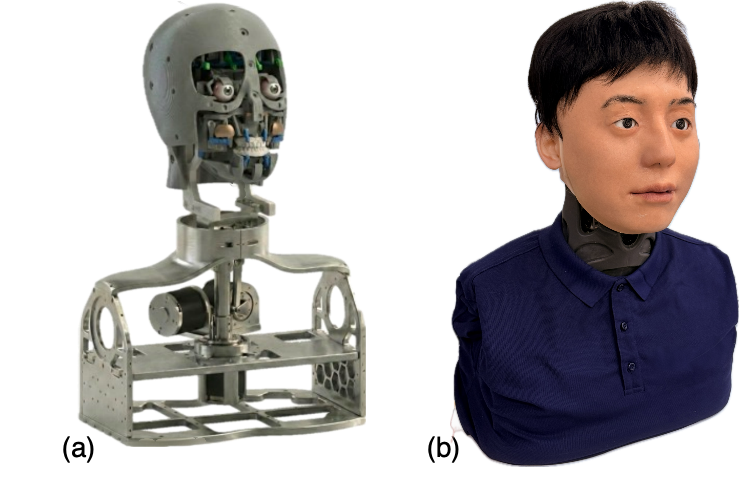
\includegraphics[width=0.82\columnwidth,keepaspectratio]{fig/fig_add.png}
    \caption{The 29-DoF facial robot platform used for the physical evaluation. \textbf{(a)}~Unskinned mechanical skeleton: servo groups span the eyelids, brows, and mouth. \textbf{(b)}~Full appearance with simulated silicone skin---the configuration driven and recorded in the experiments.}
    \label{fig:add}
\end{figure}

Experiments use the 29-DoF facial robot in Fig.~\ref{fig:add}. Control runs on an on-board Intel N100 industrial PC (4-core CPU, no discrete GPU) and issues servo commands over a serial port; generation uses Qwen2.5-0.5B throughout. The main comparison uses four conditions recorded in one session, on the same robot and camera pose, for the same reply: EmoManifold, a Mishra-style turn-level baseline~\cite{mishra2023realtime}, an Xpress-style turn-level baseline~\cite{antony2025xpress}, and a shuffled control. Table~\ref{tab:design} summarizes the design differences.

\begin{table}[t]
    \caption{Design comparison. A check denotes a property of the method as used in this paper.}
    \label{tab:design}
    \centering
    \begin{tabular}{lccc}
    \toprule
     & EmoManifold & Mishra et al. & Xpress \\
    \midrule
    Update & token & turn & turn \\
    Expression space & continuous & 6 classes & category + intensity \\
    Emotion label from the LLM & no & yes & yes \\
    External affect API & no & yes & yes \\
    Update from the first token & yes & no & no \\
    Within-utterance change & yes & no & no \\
    \bottomrule
    \end{tabular}
\end{table}

\subsection{Main Comparison}
\label{sec:exp_hardware}

\subsubsection{Actuation Fidelity}
The robot generates expression and replies live for 20 stimulus sentences. A fixed camera records the face, and an independent open-source analyzer (Py-Feat~\cite{cheong2023pyfeat}) estimates valence and arousal frame by frame. We test whether these readings change in the same direction as the commanded signal. All four conditions are recorded in one session, on the same robot and camera pose, for \emph{the same reply}. (1)~EmoManifold: VAD and the face are updated once per generated token. (2)~Mishra-style turn-level baseline~\cite{mishra2023realtime}: following the original prompt, one of six discrete emotions is assigned to the full reply and held for the turn. (3)~Xpress-style turn-level baseline~\cite{antony2025xpress}: following the official prompt, a finer emotion label with high/low intensity is assigned and held for the turn. (4)~Shuffled control: EmoManifold's per-token commands are executed after temporal shuffling, preserving amplitude but destroying order. Both baselines label replies with GPT-4o-mini, as in the original papers.

Camera readout uses Py-Feat~\cite{cheong2023pyfeat}, which is independent of our pipeline. Like other public tools of this type, Py-Feat does not provide a reliable dominance estimate. This matches the VA plane used for expression mapping (Section~\ref{sec:actuator}), so the physical evaluation covers only valence and arousal.

Because the detector is trained on human faces, applying it to a robot face introduces scale compression and cross-dimensional leakage. We fit a one-time linear calibration on 40 turn-level static segments from the Mishra/Xpress conditions, where displayed valence and arousal are known. A separate line is fit per dimension from Py-Feat readings to the known values; the parameters are then frozen for all dynamic trials and kept separate from the intra-utterance evaluation.

The primary metric is event-level directional agreement. Within each 2-s sliding window, an event is flagged when commanded valence changes by more than $0.3$ or commanded arousal by more than $0.2$. A hit is recorded if the calibrated camera readout changes in the same direction within that window (chance level $50\%$). Because windows overlap heavily, we average hit rates within each trial and bootstrap across the 20 trials for confidence intervals. We also measure the facial variance explained by EmoManifold beyond a static whole-sentence expression baseline. All four conditions share a fixed $0.5$-s actuation--detection lag.

Fig.~\ref{fig:5} shows that only EmoManifold tracks commanded transitions within the utterance: directional agreement is $87.5\%$ for valence ($95\%$ CI $[76.7,96.0]$, $p<10^{-4}$) and $69.6\%$ for arousal (CI $[56.8,81.7]$, $p{=}0.001$). Mishra, Xpress, and the shuffled control remain near the $50\%$ chance level (valence $37.2\%$--$46.5\%$, arousal $53.8\%$--$58.8\%$). A circular-shift surrogate (Fisher-combined $p<10^{-23}$) rules out chance alignment. The shuffled condition matches EmoManifold in dynamic amplitude but not in temporal order; its agreement rate and $R^2$ gain ($\le+0.05$) remain indistinguishable from the baselines, while EmoManifold explains an additional $21.8\%$/$18.9\%$ of facial variance (valence/arousal; Fig.~\ref{fig:5}c). Intra-utterance physical tracking therefore depends on command order, not merely on larger amplitude.


\begin{figure}[t]
    \centering
    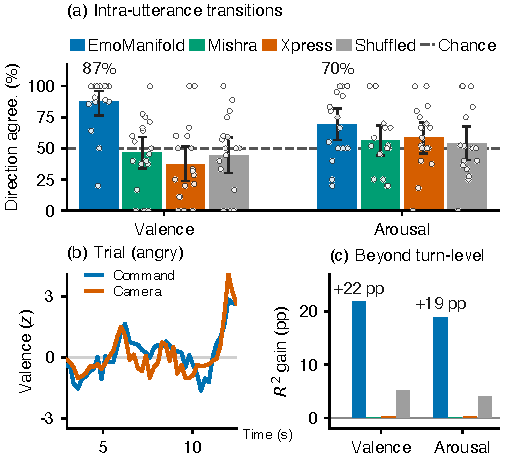
\includegraphics[width=\columnwidth,keepaspectratio]{fig/fig5.pdf}
    \caption{Token-level affective physical actuation under a same-session, four-condition comparison ($n{=}20$ replies; conditions and metrics defined in the text).
    \textbf{(a)}~Directional agreement between commanded affective transitions and camera readout within a 2-s window: bars are trial-mean with bootstrap 95\% CI, open circles are per-trial hit rates, dashed line is chance level ($50\%$).
    \textbf{(b)}~A representative trial (anger): commanded and calibrated readout trajectories after fixed-lag alignment ($z$-standardized, for display only).
    \textbf{(c)}~$R^2$ gain (percentage points) relative to the turn-level baselines.}
    \label{fig:5}
  \end{figure}


\begin{table}[t]
    \caption{On-device deployment latency (mean $\pm$ std., $n{=}20$). TTFF: time to first semantically-driven face update.}
    \label{tab:latency}
    \centering
    \resizebox{\columnwidth}{!}{%
    \begin{tabular}{lccc}
    \toprule
    System & Granularity & Per-token (ms) & TTFF (s) \\
    \midrule
    EmoManifold & token & $0.7{\pm}0.2$ & $0.96{\pm}0.19$ \\
    Mishra-style~\cite{mishra2023realtime} & turn & --- & $10.2{\pm}4.3$ / $9.9{\pm}4.0$ \\
    Xpress-style~\cite{antony2025xpress} & turn & --- & $9.9{\pm}3.8$ / $26.5{\pm}5.7$ \\
    \bottomrule
    \end{tabular}}
    \end{table}


\subsubsection{On-Device End-to-End Latency}
Table~\ref{tab:latency} reports measurements on the industrial PC. Time-to-First-Face-update (TTFF) is the main metric; for the two baselines, TTFF is measured with GPT-4o-mini (before the slash) and Qwen2.5-0.5B (after). EmoManifold's per-token computation (hidden-state projection $\to$ FKCN $\to$ EMA) takes $0.7$~ms, and the time to the first content-driven update---including the first token's forward pass---averages under 1~s. Turn-level baselines require $10$--$26$~s, not because the classifier is slow, but because they must wait for the full sentence and then run a whole-sentence classification before the first expression update. EmoManifold can update as soon as the first token is generated.


\subsection{Mechanism}
The comparison above treats the commanded signal as affect. We next check that the signal is a stable affective subspace and that it changes with context when the surface words do not.

\subsection{Reliability of the Affective Subspace}
\label{sec:exp_subspace}

\begin{figure}[t]
    \centering
    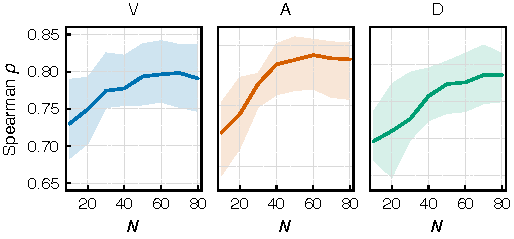
\includegraphics[width=\columnwidth]{fig/fig2.pdf}
    \caption{Word-level Spearman correlation as a function of the number of pole words $N$. Solid lines show the mean across six models; shaded bands show the min--max range. All three dimensions saturate beyond $N \approx 50$.}
    \label{fig:2}
\end{figure}

We hold out 300 evaluation words from the NRC-VAD lexicon that were not used for axis construction (100 per dimension, grouped by the most salient NRC dimension). If the $k$-th affective axis is reliable, the ranking of projections onto that axis should agree with the lexicon annotation. Concretely, we normalize each word's unembedding row, take its dot product with the corresponding axis, apply AdaptiveScaler, and compute the Spearman correlation $\rho$ against the lexicon value. To keep models comparable on the same vocabulary, we retain only words that all five comparison models (open-source LLMs from 2B to 8B) tokenize as a single token; multi-token words lack a unique unembedding row and cannot be compared fairly.

Axis quality depends on the pole-word count $N$. Fig.~\ref{fig:2} shows $\rho$ for six models on the same evaluation list as $N$ varies from 10 to 80. All three dimensions are unstable for small $N$, improve as $N$ grows, and saturate beyond $N \approx 50$; we therefore use $N{=}50$ by default. Because our deployment model, Qwen2.5, is pretrained mainly on English and Chinese~\cite{qwen2024qwen25}, we also repeat the procedure with Chinese pole words (other models' tokenizers are English-centric and rarely yield enough single-token non-English poles for a matched comparison), obtaining $\rho_V = 0.823$, $\rho_A = 0.803$, and $\rho_D = 0.702$. The same construction is thus reliable in Chinese as well.

\begin{table}[t]
    \caption{Cross-model word-level Spearman correlation ($N{=}50$).}
    \label{tab:e2_cross_model_spearman}
    \centering
    \begin{tabular}{lccc}
    \toprule
    Model & $\rho_V$ & $\rho_A$ & $\rho_D$ \\
    \midrule
    Gemma-2.2-2B & 0.802 & 0.650 & 0.598 \\
    Llama-3.2-3B & 0.800 & 0.828 & 0.708 \\
    Mistral-7B-v0.3 & 0.794 & 0.788 & 0.567 \\
    Qwen2.5-7B & 0.755 & 0.792 & 0.648 \\
    Llama-3.1-8B & 0.773 & 0.788 & 0.697 \\
    Qwen2.5-0.5B & \textbf{0.837} & 0.665 & 0.663 \\
    \bottomrule
    \end{tabular}
    \end{table}

Table~\ref{tab:e2_cross_model_spearman} reports per-dimension correlations at $N{=}50$. Three-dimension means fall in a similar range of $0.68$--$0.78$. Our deployment model, Qwen2.5-0.5B, reaches a valence correlation of $0.837$, competitive with models one to two orders of magnitude larger. Reducing the model to an edge-deployable 0.5B scale does not erase the linearly readable affective structure in hidden space.


\begin{figure}[t]
    \centering
    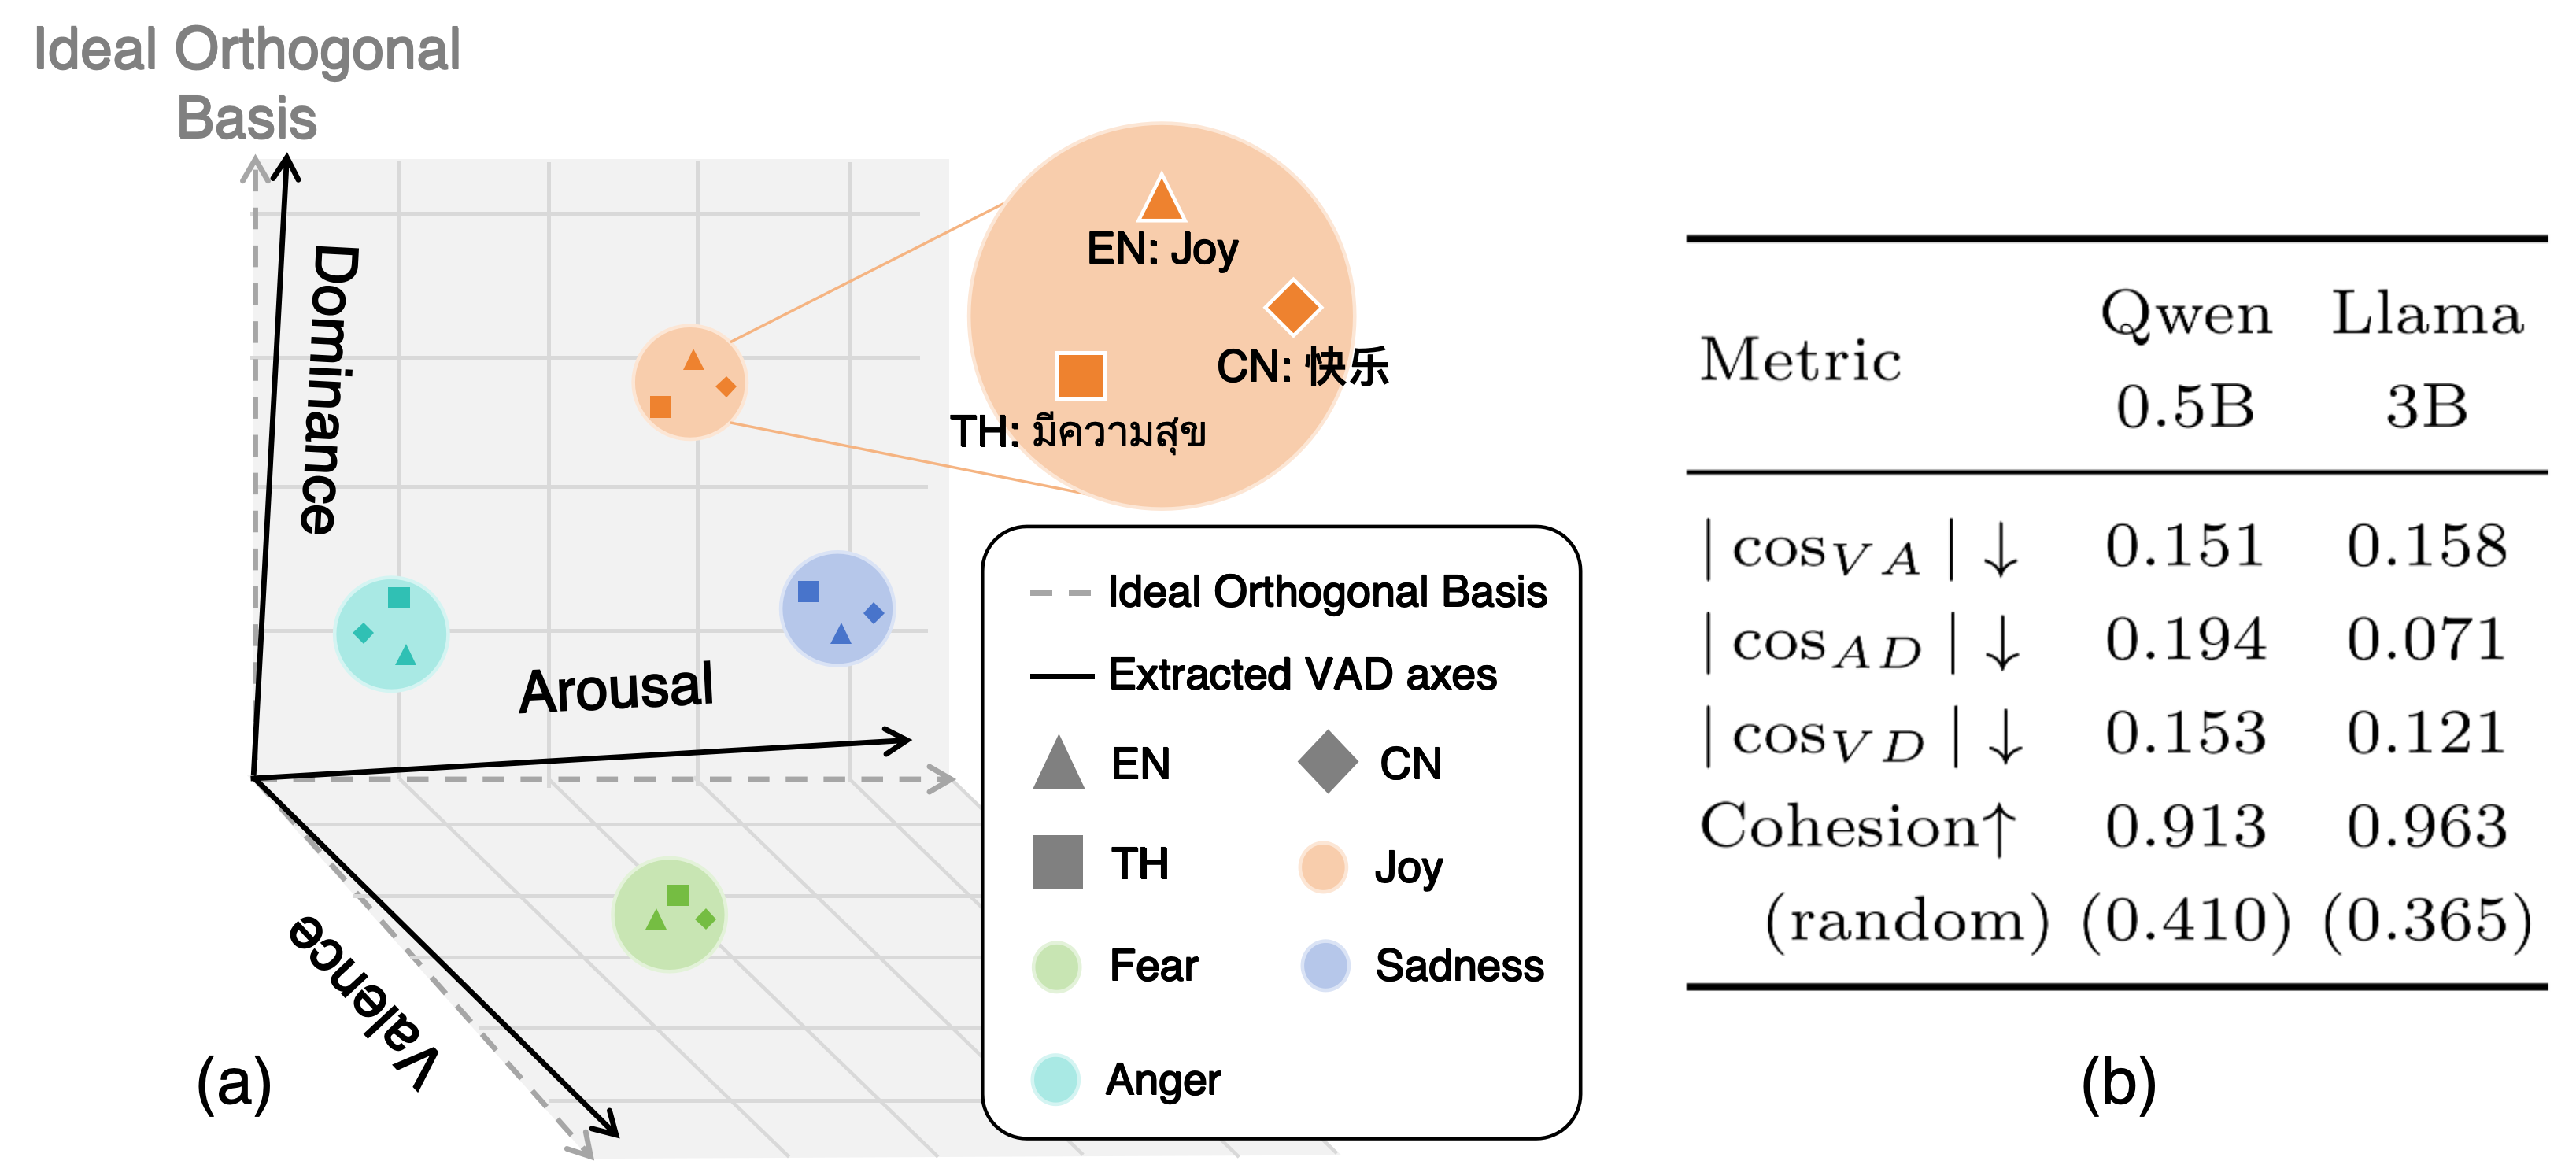
\includegraphics[width=\columnwidth]{fig/fig3.png}
    \caption{Cross-lingual affective geometry ($|\cos|$, cohesion, and the random baseline are defined in the text). \textbf{(a)}~Schematic of cross-lingual emotion word clusters (illustrative, not measured): solid lines are the three mined affective axes; dashed lines are an idealized orthogonal basis. \textbf{(b)}~Quantitative results after each backbone independently constructs its axes from English pole words ($N{=}50$); parenthesized numbers are the random baseline on the corresponding model, matching the cohesion trend in (a).}
    \label{fig:3}
\end{figure}

Section~\ref{sec:exp_subspace} established per-dimension reliability. Downstream use---direct readout or distance-based expression mapping (Section~\ref{sec:actuator})---also requires that the three axes be approximately non-overlapping in direction, and that this geometry not be an artifact of one model or language. On Qwen2.5-0.5B and Llama-3.2-3B (Table~\ref{tab:e2_cross_model_spearman}), we therefore build axes independently from English pole words ($N{=}50$) and measure inter-axis orthogonality. We also prepare five cross-lingual emotion clusters (fear, comfort, dominance, strength, calm), each with synonyms in English, Chinese, and three additional languages drawn from Spanish, Polish, Portuguese, Arabic, Italian, Dutch, German, French, and Japanese. Every word is a single token under its \emph{corresponding} model's tokenizer. We project each word into the mined VAD subspace and compute mean pairwise cosine similarity within each cluster, using the same statistic on a random three-dimensional orthogonal basis (100 trials per cluster) as a negative control. Fig.~\ref{fig:3}a sketches the intended geometry; Fig.~\ref{fig:3}b reports quantitative results for English-built axes: on Qwen, $|\cos|\le0.194$ and cohesion is $0.913$ (random: $0.410$); on Llama, $|\cos|\le0.158$ and cohesion is $0.963$ (random: $0.365$). To test generality rather than a single deployment setting, we also rebuild axes from Chinese pole words on both models. Llama's English-centric tokenizer fragments Chinese more readily and yields fewer usable single-token poles, yet the results remain comparable: $|\cos|\le0.220$ and cohesion $0.898$ on Qwen, and $|\cos|\le0.282$ and cohesion $0.965$ on Llama. The cross-lingual geometry therefore holds across both models and both languages.


\subsection{Context Sensitivity}
\label{sec:exp_sarcasm}

\begin{figure}[t]
    \centering
    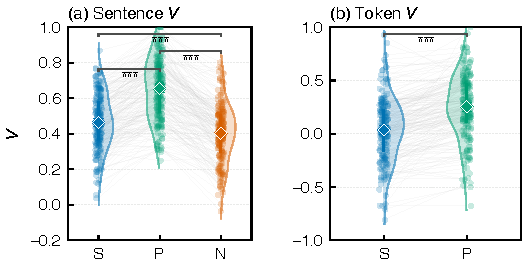
\includegraphics[width=\columnwidth]{fig/fig4.pdf}
    \caption{Contextual-triplet sarcasm stress test ($n{=}200$, Qwen2.5-0.5B; triplet construction in the text).
    \textbf{(a)}~Sentence-level projected valence $V$ for S (sarcastic), P (sincere-positive), and N (literal-negative). Raincloud plots combine a half-violin (kernel density), a box plot (IQR), and per-triplet scatter points; diamonds are bootstrap means $\pm$95\% CI, gray lines connect matched triplets.
    \textbf{(b)}~Token-level valence at the primary anchored positive keyword, S versus P ($n{=}194$).}
    \label{fig:4}
  \end{figure}

Word-level correlations show agreement with lexicon priors, but not whether the readout integrates context. If the readout were little more than a dictionary lookup, the same positive wording would receive similarly high valence regardless of context, and expression could not track intra-utterance pragmatic shifts. Sarcasm is a strong test case: a sarcastic sentence conveys negative intent with positive wording, so surface lexicon and true affective direction conflict~\cite{abufarha2022isarcasm}.

We start from the English SubTask~C set of iSarcasmEval~\cite{abufarha2022isarcasm}, which provides 200 pairs of a sarcastic sentence and a non-sarcastic rephrasing with the same intent. Using the raw sentences has two problems: many depend on culture-specific references (sports teams, politicians, brands), and an isolated quotation lacks the situation needed to judge sarcasm. We therefore rewrite each pair into a contextual triplet under a fixed protocol. Each item is one sentence of observable context plus one quoted utterance, with culture-specific references replaced by everyday scenarios. S (sarcastic) pairs adverse context with a positive quotation; P (sincere-positive) pairs favorable context with a quotation that is \emph{word-for-word identical} to S; N (literal-negative) pairs the same adverse context with a negative quotation. For example, S and P share \emph{``Your team played so well today!''}, differing only in whether the preceding context is a loss or a win; in N the quotation is rewritten to be literally negative. Because S and P share identical quotations, any projection difference must come from context. We also annotate 1--3 anchored emotion keywords per triplet (e.g., ``well'') for token-level analysis.

For each triplet we use the same forward projection as elsewhere: sentence-level valence at the final token, and keyword-level valence at the anchored keyword. Fig.~\ref{fig:4}a shows that, across 200 triplets, sentence-level valence for S and N overlaps extensively ($81.5\%$ of pairs differ by less than $0.15$), while S is significantly lower than P despite an identical quotation ($\Delta V=-0.19$; Wilcoxon, $n{=}200$, $p<10^{-11}$). All three pairwise comparisons are significant.

A sentence-level gap could still be driven by other words. We therefore restrict the comparison to a single token: the same positive keyword (e.g., ``well'') appears in the same position and surface form in S and P, with only the preceding context changing. Fig.~\ref{fig:4}b reports token-level valence at the primary anchored keyword: it is $0.22$ lower under sarcasm on average ($-0.20$ across all co-occurring keywords), while arousal and dominance shifts remain below $0.07$. The change is almost entirely in valence, consistent with sarcasm as a shift in evaluation rather than arousal~\cite{leggitt2000emotional}. Because surface form and position are matched, the valence difference must come from context, indicating context-integrated affect rather than dictionary-style matching. Repeating the analysis on Llama-3.2-3B with the same triplets and axis-construction protocol yields sentence-level $\Delta V(S{-}P){=}-0.20$ and a primary-keyword difference of $-0.16$, matching Qwen in direction and magnitude. The effect is therefore not specific to the 0.5B deployment model.

%%%%%%%%%%%%%%%%%%%%%%%%%%%%%%%%%%%%%%%%%%%%%%%%%%%%%%%%%%%%%%%%%%%%%%%%%%%%%%%%

\subsection{Robustness}
\subsubsection{Hyperparameter Robustness}
The main comparison uses default EMA coefficient $\alpha{=}0.6$ and prototype count $P{=}13$. These hyperparameters affect only the deterministic command-side computation; servos, camera, and detector are shared across settings. We therefore offline-replay the full display pipeline (FKCN $\to$ EMA $\to$ 10\,fps ease-in--ease-out interpolation $\to$ per-frame rate limit) on the same 20 commanded trajectories, with the same event thresholds and windows, instead of re-recording physical video for every setting. Under the default setting, replay yields $84.4\%$ valence and $67.7\%$ arousal agreement, close to the camera-measured $87.5\%$/$69.6\%$. The same pipeline on time-shuffled commands yields only $44\%$--$48\%$ (arousal $40\%$--$45\%$), so the metric is not trivially high. Sweeping $\alpha\in\{0.3,0.6,0.9\}$ against default $P{=}13$ and two $P{=}7$ constructions (each retaining a different prototype per class) gives nine settings in total: valence agreement is $75\%$--$87\%$ and arousal agreement is $68\%$--$74\%$, both well above the shuffled floor. Intra-utterance actionability is therefore not driven by these hyperparameters.


\begin{figure}[t]
  \centering
  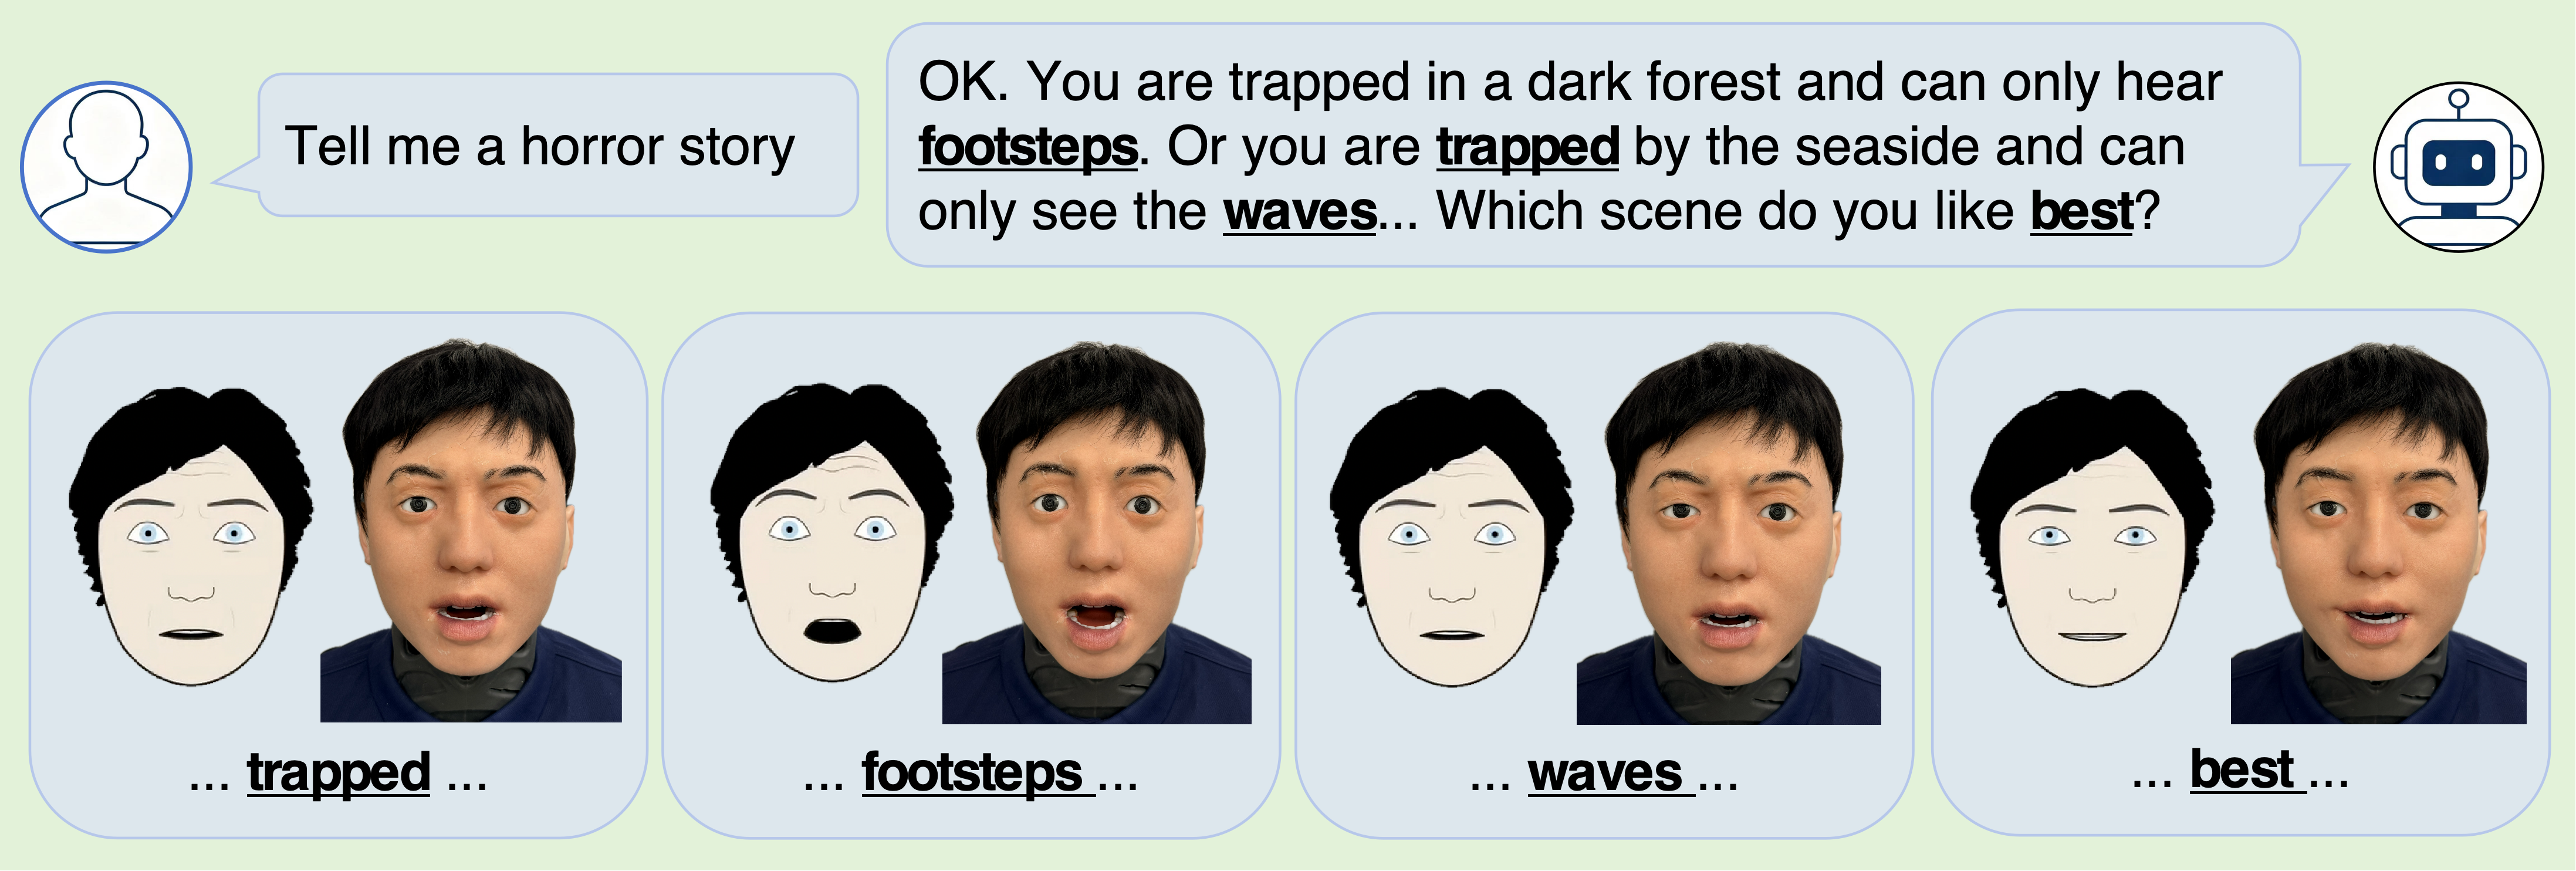
\includegraphics[width=\columnwidth,keepaspectratio]{fig/fig7.png}
  \caption{Dual-carrier expression synchronization under a streaming reply (schematic). Top: dialogue with four sampled tokens underlined for illustration; bottom: Grimace simulated face (left) and physical face (right) at the corresponding time points.}
  \label{fig:7}
\end{figure}


As a qualitative check of carrier transfer, Fig.~\ref{fig:7} compares the Grimace simulated face and the physical face on the same dialogue at matched time points; both carriers show consistent expression changes, supporting the platform-agnostic fusion-weight design in Section~\ref{sec:actuator}.

\subsection{Human Study}
Camera readout shows whether the physical face tracks the command, but not whether observers recognize the expressions or prefer token-level dynamics. We therefore ran two silent-video questionnaires ($n{=}20$). Participants gave informed consent; responses were anonymous and contained no personally identifiable information.

First, we ask whether expressions can be identified correctly. The model generates replies targeting a given emotion; participants watch EmoManifold-driven videos and judge the emotion category. Accuracy is compared with \emph{hand-tuned reference expressions} recorded at the same camera pose, which approximate the hardware's recognition ceiling. EmoManifold reaches $85.5\%$ accuracy versus $90.5\%$ for the references (Wilcoxon $p{=}0.013$), a modest gap. Confusions in both systems concentrate on inherently similar pairs such as fear--surprise and sadness--disgust, suggesting that the residual gap reflects the robot face's expressive limits rather than mis-mapped emotions.

Second, we ask whether token-level dynamic expression is preferred. For sentences with an intra-utterance emotional shift, participants choose among three videos---EmoManifold's dynamic expression, a single expression held for the whole sentence, and the shuffled-order control---the one that ``best matches the emotional change.'' EmoManifold is chosen $83.5\%$ of the time, versus $11.5\%$ for the shuffled control and $5.0\%$ for the static expression (all 20 participants preferred EmoManifold; one-sided Wilcoxon $p<10^{-6}$). Intra-utterance dynamic expression is therefore both recognizable and preferred.

%%%%%%%%%%%%%%%%%%%%%%%%%%%%%%%%%%%%%%%%%%%%%%%%%%%%%%%%%%%%%%%%%%%%%%%%%%%%%%%%
\section{DISCUSSION}
\label{sec:discussion}

Taken together, the three experiments form a single chain of evidence: the mined VAD subspace is linearly readable across models and languages; the same readout shifts with pragmatic context rather than surface wording; and, once mapped through FKCN and presets, the resulting commands are recoverable on a physical face and preferred by observers over turn-level or temporally shuffled controls. Relative to turn-level discrete sentence labels, the main practical gain is temporal: expression can track intra-utterance valence and arousal changes instead of waiting for a whole-reply category.

Beyond these results, several limitations remain. Our evaluations establish expression--content alignment at token rate; what remains open is coupling that channel to audible playback. Human studies use silent video, so we do not claim expression--audio synchrony, and the system does not yet drive audio-synchronized lip motion. Mouth DoFs must serve both articulation and expression, and naive superposition can interfere. A natural next step---which we are exploring---is to apply the same hidden-state readout to open-source speech-native models and project affect along the audio-token stream, so facial updates can share the playback clock; lip articulation can then be handled as a complementary controller on that shared timeline.

Second, the face hardware and the interaction policy both constrain what can be shown. Discrimination among neighboring emotions is limited by the robot's physical DoFs and preset expression basis. More critically, directly externalizing an internal affective state may be inappropriate in some settings: human social interaction often requires suppressing, softening, or delaying expression, whereas the current pipeline displays the signal as soon as it is read. We therefore plan a lightweight, optional regulation stage between projection and actuation---gain limiting, temporal hold, and an explicit off switch---so deployment can choose when the internal signal should be shown, softened, or suppressed.

Third, the physical and human studies remain modest in scale (corpus size, participant count, and platform). Participants gave informed consent (Section~\ref{sec:exp_hardware}); larger-sample replication is left to future work. The physical actuation and human-evaluation study (Section~\ref{sec:exp_hardware}) also uses only Qwen2.5-0.5B. Because the subspace and context-sensitivity experiments already show comparable geometry and sensitivity on Llama-3.2-3B, we concentrated hardware and human-evaluation resources on the deployment model. Repeating the full closed-loop protocol on a second backbone, with a larger participant pool, is the direct next measurement step along the same evaluation pipeline.

\section{CONCLUSION}
\label{sec:conclusion}

This paper shows that a facial robot need not rely on a discrete, whole-sentence emotion label. Continuous VAD coordinates can be read from an LLM's hidden states during streaming decoding and used to drive physical expression at token granularity. Across experiments, the training-free pipeline yields a context-sensitive VAD readout, tracks commanded intra-utterance valence--arousal transitions on a physical face more faithfully than turn-level baselines, and reduces end-to-end expression-response latency, offering a practical route beyond turn-level control toward fast, fine-grained, and verifiable embodied affective interaction.

\bibliographystyle{IEEEtran}
\bibliography{references_en}

\end{document}
